\documentclass[runningheads]{llncs}

\usepackage[T1]{fontenc}
\usepackage[utf8]{inputenc}
\usepackage[spanish,provide=*]{babel}
\usepackage{amsmath,amssymb}
\usepackage{graphicx}
\usepackage{booktabs}
\usepackage{microtype}
\usepackage{array}
\usepackage{multirow}
\usepackage{enumitem}
\setlist{noitemsep, topsep=2pt}
\usepackage{hyperref}

% Compactación de espacio para ajustar a 10 páginas (LLNCS, 1 columna)
\renewcommand{\arraystretch}{0.95}
\setlength{\textfloatsep}{8pt plus 2pt minus 2pt}
\setlength{\intextsep}{8pt plus 2pt minus 2pt}
\emergencystretch=3em  % evita overfull \hbox en párrafos con tokens largos (\texttt)

\hypersetup{
  colorlinks=true,
  linkcolor=black,
  citecolor=black,
  urlcolor=black
}

% -----------------------------------------------------------------------
\title{pico-JEPA v2: ¿Cuándo Superan Muchos\\
Modelos Pequeños a Uno Grande?}
\titlerunning{pico-JEPA v2}

\author{Adrián Rostagno \and Javier Iparraguirre \and Roberto Briatore \and
Agustín González \and Santiago Aggio}
\authorrunning{A. Rostagno et al.}
\institute{Universidad Tecnológica Nacional, Facultad Regional Bahía Blanca,
Bahía Blanca, Argentina\\
\email{\{arostag, jiparraguirre, rbriatore, agonzalez, slaggio\}@frbb.utn.edu.ar}}

\begin{document}

\maketitle

% -----------------------------------------------------------------------
\begin{abstract}
pico-JEPA es un sistema que aprende a representar videos sin necesidad de
etiquetas, pensado para correr en una computadora de escritorio. En esta segunda
versión, pico-JEPA v2, ponemos a prueba una idea sencilla: en lugar de entrenar
un único modelo grande con todos los datos, entrenar varios modelos pequeños
---cada uno con una porción distinta--- y combinar sus predicciones puede dar
mejor exactitud. Evaluamos esta idea sobre 30 clases de Kinetics-700, con una red
base ViT compacta ($\approx 3.4$M de parámetros) entrenada sin etiquetas sobre
3\,000 videos en una sola placa gráfica de escritorio. Al diversificar la
arquitectura del clasificador entre los miembros del conjunto y combinarlos
mediante \emph{apilamiento}, el conjunto supera al modelo único con significancia
estadística formal (una ventaja de $+5.10$\,pp sobre el conjunto reservado, con
un intervalo de confianza del 95\,\% que excluye el cero y se mantiene ante
distintas semillas); las nueve configuraciones evaluadas durante la búsqueda
favorecen al conjunto. Dos experimentos controlados delimitan cuándo vale la
idea: la ventaja desaparece con redes base de menor capacidad o con pocas clases.
Más que una validación de sí o no, nuestra contribución central es un
\emph{mapa de condiciones} ---capacidad de la red base, cantidad de clases y
forma de combinar las predicciones--- bajo las cuales la sabiduría colectiva de
modelos pequeños supera al modelo único, en un escenario de cómputo y datos
deliberadamente acotado.

\keywords{aprendizaje auto-supervisado de video \and conjuntos de modelos \and
apilamiento \and JEPA \and ViT \and Kinetics-700}
\end{abstract}

% -----------------------------------------------------------------------
\section{Introducción}

Enseñar a una computadora a entender videos suele exigir grandes cantidades de
material etiquetado a mano, una tarea costosa y lenta. El aprendizaje
auto-supervisado ofrece una alternativa: el modelo aprende mirando videos sin
etiquetas. Dentro de esta familia, la arquitectura JEPA~\cite{lecun2022path}
aprende a predecir cómo se ve una región oculta del video a partir de la región
visible, sin reconstruir cada pixel, y así obtiene representaciones más abstractas
y útiles~\cite{assran2023self}.

En este trabajo abordamos una pregunta complementaria: dado un presupuesto fijo de
cómputo y datos, ¿conviene entrenar un único modelo grande con todo el material, o
varios modelos pequeños, cada uno con una porción distinta, y luego combinar sus
predicciones? Esta es la hipótesis central de \emph{pico-JEPA}~\cite{rostagno2025pico}.

La intuición proviene del refrán «la unión hace la fuerza»: si cada modelo se
equivoca de manera distinta, la decisión conjunta puede ser más acertada que la de
cualquiera por separado~\cite{dietterich2000ensemble,lakshminarayanan2017simple}.
Sin embargo, esta ventaja no es automática: depende de la capacidad de cada
modelo, de la calidad de lo aprendido y de cómo se combinen las
predicciones~\cite{wenzel2020hyperparameter}.

Respecto de nuestro trabajo previo~\cite{rostagno2025pico}, que mostró la
viabilidad de pico-JEPA en hardware de escritorio con votación simple sobre pocas
clases, esta versión aporta cuatro elementos nuevos: (a) un conjunto
\emph{heterogéneo}, en el que cada modelo lleva una cabeza de clasificación
distinta; (b) el \emph{apilamiento} como forma de combinar las predicciones;
(c) un análisis estadístico formal con remuestreo \emph{bootstrap} y verificación
de robustez ante distintas semillas; y (d) la caracterización de las
\emph{condiciones de validez} de la hipótesis mediante experimentos controlados.
Concretamente, nuestras contribuciones son:
\begin{enumerate}
  \item Un flujo de trabajo completo de pico-JEPA v2: entrenamiento sin etiquetas
        seguido de clasificación supervisada con conjunto heterogéneo, ejecutable
        íntegramente en una placa gráfica de escritorio.
  \item La validación experimental de la hipótesis principal sobre K700-val, con
        significancia formal vía bootstrap para la combinación por apilamiento.
  \item \textbf{La caracterización de las condiciones de validez}: dos
        experimentos controlados (capacidad de la red base y cantidad de clases)
        que delimitan \emph{cuándo} la ventaja del conjunto aparece y cuándo
        desaparece ---un mapa de validez más informativo que una afirmación de
        sí o no.
  \item El análisis de cuatro formas de combinar predicciones y la evidencia de
        que el \emph{apilamiento} es necesario para convertir la diversidad de los
        modelos en una mejora medible.
\end{enumerate}

% -----------------------------------------------------------------------
\section{Trabajo Relacionado}

V-JEPA~\cite{bardes2024revisiting} extiende I-JEPA~\cite{assran2023self} al
dominio temporal: oculta bloques de información que abarcan varios cuadros a la
vez (los llamados \emph{tubelets}, o tubos espacio-temporales) y aprende a
predecir su contenido con un codificador de contexto y un codificador objetivo
que se actualiza lentamente, sin reconstruir pixeles. Nuestro trabajo
previo~\cite{rostagno2025pico} adoptó esta formulación en hardware de escritorio;
aquí la extendemos con un conjunto heterogéneo y un análisis estadístico formal.

Combinar varias redes profundas mejora la confiabilidad y la robustez de las
predicciones~\cite{lakshminarayanan2017simple}. La diversidad entre los modelos
puede provenir de distintas inicializaciones~\cite{fort2019deep}, de darle a cada
uno una porción distinta de los datos, de variar su arquitectura, o de variar sus
hiperparámetros, que aporta beneficios análogos~\cite{wenzel2020hyperparameter}.
En video es habitual promediar la predicción sobre varios fragmentos del mismo
clip para obtener evaluaciones más estables~\cite{wang2018temporal}. La idea de
que cada modelo se especialice en una parte distinta del problema se remonta a las
mezclas de expertos~\cite{jacobs1991adaptive}; a diferencia de aquellas, donde un
mecanismo aprendido decide qué experto usar, pico-JEPA reparte las clases de forma
explícita y equilibrada, lo que hace la especialización transparente y fácil de
controlar.

% -----------------------------------------------------------------------
\section{Arquitectura de pico-JEPA v2}
\label{sec:arch}

\subsection{Entrenamiento sin Etiquetas}

El entrenamiento sin etiquetas sigue la receta de JEPA para video. Cada clip
$\mathbf{v} \in \mathbb{R}^{C \times T \times H \times W}$ se parte en parches
espacio-temporales de tamaño $(t, h, w) = (2, 16, 16)$, lo que produce
$N_p = (T/t)\times(H/h)\times(W/w) = 4{\times}14{\times}14 = 784$ parches.

De esos parches, una parte se mantiene visible (el \emph{contexto}, un 20\,\% de
los parches) y el resto se oculta (el \emph{objetivo}, un 80\,\%). El sistema
entrena dos codificadores y un predictor:

\begin{itemize}
  \item \textbf{Codificador en línea} $f_\theta$: una red ViT reducida ($d{=}192$,
        la mitad del ViT-Small canónico de $d{=}384$) que procesa el clip con los
        parches de contexto visibles.
  \item \textbf{Codificador objetivo} $f_{\bar\theta}$: la misma red, pero sus
        pesos no se ajustan por descenso de gradiente, sino como un promedio móvil
        de los del codificador en línea:
        $\bar\theta \leftarrow \tau\bar\theta + (1{-}\tau)\theta$, con $\tau$
        siguiendo un esquema cosenoidal de $0.996$ a $0.9999$.
  \item \textbf{Predictor} $g_\phi$: una red más superficial que, a partir del
        contexto, predice la representación de los parches ocultos $\hat{z}_i$.
\end{itemize}

El modelo aprende minimizando el error cuadrático medio entre lo que predice y lo
que produce el codificador objetivo:
\begin{equation}
  \mathcal{L} = \frac{1}{|\mathcal{T}|}\sum_{i \in \mathcal{T}}
  \bigl\|\hat{z}_i - \mathrm{sg}\!\left[f_{\bar\theta}(\mathbf{v})_i\right]\bigr\|_2^2
  \label{eq:loss}
\end{equation}
donde $\mathrm{sg}[\cdot]$ indica que el codificador objetivo no recibe gradiente
(su único cambio viene del promedio móvil). Este detalle es esencial: sin él,
ambos codificadores colapsarían a una representación trivial y constante.

\subsection{Clasificación Supervisada}

Una vez entrenado el codificador $f_\theta$, le agregamos una cabeza de
clasificación, que puede ser de tres tipos:
\begin{itemize}
  \item \textbf{Lineal}: una capa lineal sobre el promedio de los parches.
  \item \textbf{MLP de 2 capas}: dos capas con una no linealidad ReLU.
  \item \textbf{Atencional}: una capa de atención entre parches seguida de una
        capa lineal, que recupera mejor la estructura temporal del video.
\end{itemize}

El codificador puede mantenerse congelado (\texttt{freeze\_encoder=True}) o
ajustarse finamente con una tasa de aprendizaje pequeña
($\text{lr\_codificador} = 3{\times}10^{-5}$,
$\text{lr\_cabeza} = 5{\times}10^{-4}$).

\subsection{El Conjunto y la Combinación de Predicciones}

El sistema entrena $N=4$ modelos pequeños (que llamaremos \emph{submodelos}). Cada
uno recibe una porción distinta de los datos, repartida de forma equilibrada entre
clases (\texttt{stratified-by-class}). Para que los submodelos no aprendan
exactamente lo mismo, los hacemos diversos en varios aspectos:

\begin{itemize}
  \item Tipo de cabeza (\texttt{head\_type}): se rota entre lineal, MLP de 2 capas
        y atencional.
  \item Congelar o no el codificador (\texttt{freeze\_encoder}): se alterna.
  \item Tasa de aprendizaje de la cabeza (\texttt{learning\_rate\_classifier}):
        con una perturbación aleatoria de $\pm$30\,\%.
  \item Semilla aleatoria (\texttt{seed}): distinta en cada submodelo
        ($\text{semilla\_base} + 1000 \cdot i$).
  \item Cantidad de épocas (\texttt{num\_epochs\_classify}): la base $\pm 2$.
\end{itemize}

Para combinar las predicciones de los cuatro submodelos comparamos cuatro
estrategias:
\begin{enumerate}
  \item \textbf{Votación dura}: gana la clase más votada.
  \item \textbf{Votación blanda}: se promedian las probabilidades softmax.
  \item \textbf{Votación ponderada}: el promedio da más peso a los submodelos que
        mejor rindieron en validación.
  \item \textbf{Apilamiento}: un meta-modelo (una regresión logística) se entrena
        sobre las $N \times C$ probabilidades de todos los submodelos y aprende a
        ponderar a cada uno según convenga.
\end{enumerate}

% -----------------------------------------------------------------------
\section{Configuración Experimental}

\subsection{Datos}

Usamos Kinetics-700-2020 (K700)~\cite{smaira2020short}, un conjunto público de
reconocimiento de acciones humanas en video. En lo que sigue, ``K700-val'' denota
su partición de validación.

\begin{itemize}
  \item \textbf{Entrenamiento sin etiquetas}: 3\,000 videos de la partición
        \texttt{train/}, sin usar sus etiquetas.
  \item \textbf{Clasificación}: 30 clases de la partición \texttt{val/},
        1\,467 videos en total.
  \item \textbf{Partición} (fija, semilla=1337): entrenamiento\,876 /
        validación\,297 / \textbf{conjunto reservado\,294}.
\end{itemize}

Los videos se procesan como clips de 8 cuadros ($224{\times}224$ pixeles),
normalizados con las estadísticas de ImageNet. La lectura de video usa
torchcodec~v0.4.0 sobre FFmpeg~v6.

Al evaluar usamos \emph{evaluación con múltiples fragmentos}: de cada video se
toman $n_\text{frag}{=}10$ clips y se promedian sus probabilidades antes de
decidir la clase. Esto reduce la variabilidad de la predicción y es práctica
habitual en reconocimiento de acciones en video~\cite{wang2018temporal}.

\subsection{Arquitectura e Hiperparámetros}

El codificador es una red ViT reducida ($d{=}192$, profundidad 8, 8 cabezas de
atención, parche $(2{,}16{,}16)$, 784 parches, $\approx$3.4M de parámetros). La
Tabla~\ref{tab:hyperparams} resume el resto de los hiperparámetros del sistema.

\begin{table}[h]
\centering
\caption{Hiperparámetros del entrenamiento sin etiquetas y del conjunto.}
\label{tab:hyperparams}
\setlength{\tabcolsep}{4pt}
\begin{tabular}{@{}llll@{}}
\toprule
\multicolumn{2}{@{}l}{\textit{Entrenamiento sin etiquetas}} & \multicolumn{2}{l}{\textit{Conjunto}}\\
Épocas & 20 & $N$ submodelos & 4\\
Fracción oculta & 0.80 & Fragmentos/video & 10\\
Ocultamiento & Multibloque (3) & Reparto & equilibrado por clase\\
Promedio móvil $[\tau_0,\tau_1]$ & $[0.996, 0.9999]$ & & \\
Decaimiento por capa & 0.9 & & \\
\bottomrule
\end{tabular}
\end{table}

\subsection{Cómo Medimos el Éxito}

La medida principal es la \emph{brecha}: cuánto supera (en puntos porcentuales,
pp) la exactitud del conjunto a la del modelo único sobre el conjunto reservado:
\begin{equation}
  \Delta = \text{exactitud}_\text{conjunto}(\mathcal{H}) -
           \text{exactitud}_\text{único}(\mathcal{H})
  \label{eq:gap}
\end{equation}
donde $\mathcal{H}$ es el conjunto reservado (294 videos). Para saber si la brecha
es real o producto del azar, estimamos un intervalo de confianza (IC) del 95\,\%
mediante remuestreo bootstrap sobre $\mathcal{H}$ ($n{=}10\,000$ remuestreos,
semilla=1337); $\text{CI}_\text{low}$ y $\text{CI}_\text{high}$ son sus extremos
inferior y superior. El veredicto depende de dónde cae el intervalo respecto del
cero: \textbf{SOPORTADO} si $\text{CI}_\text{low} > 0$ (todo el intervalo queda
por encima de cero, es decir, el conjunto supera al modelo único con un 95\,\% de
confianza); \textbf{INCONCLUSO} si la brecha es positiva pero el intervalo
contiene el cero; y \textbf{RECHAZADO} si la brecha no es positiva.

El modelo único ---nuestra referencia--- se entrena con los 876 videos de
entrenamiento completos. La comparación responde a la hipótesis tal como se
plantea ---muchos modelos pequeños sobre porciones frente a un único modelo sobre
todos los datos--- y no iguala explícitamente el presupuesto de cómputo: el
conjunto cuesta $N$ veces el entrenamiento del modelo único. Una comparación a
igual cantidad de operaciones es una extensión natural de este protocolo.

El hardware utilizado fue: Intel Core i7, 65\,GB de RAM y una placa NVIDIA GTX
1060 de 6\,GB.

\paragraph{Reproducibilidad.} Todo el protocolo es determinístico: la triple
partición (entrenamiento/validación/reservado) se genera con \texttt{semilla=1337}
y queda fija durante toda la búsqueda, de modo que el conjunto reservado permanece
intocado hasta la evaluación final. El código, las configuraciones y los programas
de evaluación estarán disponibles para revisión.

% -----------------------------------------------------------------------
\section{Resultados}

\subsection{Las Nueve Mediciones de la Fase 4}

El flujo de trabajo de pico-JEPA se organiza en cuatro fases que un bucle de
búsqueda recorre de manera iterativa: (1)~entrenamiento sin etiquetas del
codificador; (2)~entrenamiento de los clasificadores (los $N$ submodelos del
conjunto y el modelo único); (3)~combinación del conjunto; y (4)~evaluación de la
hipótesis sobre el conjunto reservado. Las tres primeras corresponden a los
componentes descritos en la Sección~\ref{sec:arch}; la \textbf{Fase 4} es la única
que accede al conjunto reservado y mide la métrica oficial, la brecha de la
Ec.~\eqref{eq:gap}. El bucle propone configuraciones sucesivas del clasificador y
del conjunto, y cada vez que la combinación mejora en validación dispara una
evaluación de Fase 4. Las nueve mediciones que siguen son precisamente esas
evaluaciones en puntos sucesivos del recorrido, con el modelo único en distintos
grados de entrenamiento.

\begin{table}[h]
\centering
\caption{Mediciones de la Fase 4 con conjunto heterogéneo ($N=4$). Las nueve
tienen brecha positiva.}
\label{tab:phase4}
\setlength{\tabcolsep}{4pt}
\begin{tabular}{cccccc}
\toprule
\textbf{Id} & \textbf{Brecha (pp)} & \textbf{CI$_\text{low}$} & \textbf{CI$_\text{high}$}
            & $\text{exact}_\text{conj}$ & $\text{exact}_\text{únic}$ \\
\midrule
8  & $+3.40$ & $-0.34$ & $+6.80$ & 9.52\,\% & 6.12\,\% \\
9  & $+3.40$ & $-0.34$ & $+7.14$ & 9.52\,\% & 6.12\,\% \\
\textbf{10} & $\mathbf{+4.08}$ & $\mathbf{+0.68}$ & $+7.82$
            & 10.20\,\% & 6.12\,\% \\
11 & $+2.72$ & $-1.02$ & $+6.46$ & 8.84\,\% & 6.12\,\% \\
13 & $+1.02$ & $-2.72$ & $+4.76$ & 9.52\,\% & 8.50\,\% \\
16 & $+2.72$ & $-1.36$ & $+6.46$ & 10.20\,\% & 7.48\,\% \\
32 & $+2.04$ & $-2.04$ & $+6.12$ & 10.20\,\% & 8.16\,\% \\
37 & $+1.02$ & $-3.06$ & $+5.10$ & 10.88\,\% & 9.86\,\% \\
42 & $+2.38$ & $-1.37$ & $+6.46$ & 10.54\,\% & 8.16\,\% \\
\midrule
\multicolumn{2}{l}{\textit{Promedio}} &
  \multicolumn{2}{l}{$+2.53$\,pp} & & \\
\bottomrule
\end{tabular}
\end{table}

Las 9 mediciones de la Tabla~\ref{tab:phase4} son todas estrictamente positivas.
Si la verdadera brecha fuera cero, obtener nueve positivos seguidos sería tan
improbable como sacar nueve caras seguidas con una moneda:
\begin{equation}
  P(9/9\ \text{positivos} \mid H_0) = 0.5^9 = \tfrac{1}{512} \approx 0.002.
  \label{eq:signtest}
\end{equation}

El promedio de las nueve es $\bar\Delta = +2.53$\,pp. Ahora bien, estas mediciones
\emph{no son estadísticamente independientes}: comparten el mismo conjunto
reservado y provienen de configuraciones sucesivas del mismo bucle de búsqueda.
Por eso no reportamos un intervalo de confianza sobre este promedio; la prueba de
signos y el promedio deben leerse como evidencia de la \textbf{consistencia
direccional} del efecto (las nueve configuraciones favorecen al conjunto), no como
una prueba formal de significancia, que requeriría mediciones independientes. La
evidencia formal proviene del bootstrap sobre el conjunto reservado para una
combinación fija (Sección~\ref{sec:agg}), reforzada por su robustez ante distintas
semillas.

\subsection{Cómo Conviene Combinar las Predicciones}
\label{sec:agg}

La Tabla~\ref{tab:aggregations} y la Fig.~\ref{fig:aggregations} comparan las
cuatro estrategias sobre el mismo conjunto reservado, en un experimento controlado
independiente del bucle de búsqueda: se fija un conjunto de submodelos y un modelo
único (con $\text{exact}_\text{únic}=6.80\,\%$), y solo se varía la forma de
combinar. Por eso las exactitudes absolutas de esta tabla
($\text{exact}_\text{conj}=11.90\,\%$ para apilamiento) no son directamente
comparables con los puntos individuales de la Tabla~\ref{tab:phase4}, que
corresponden a distintas configuraciones del recorrido.

\begin{table}[h]
\centering
\caption{Comparación de formas de combinar predicciones (4 submodelos
heterogéneos, $\text{exact}_\text{únic} = 6.80\,\%$).}
\label{tab:aggregations}
\begin{tabular}{lcccc}
\toprule
\textbf{Combinación} & $\text{exact}_\text{conj}$ & \textbf{Brecha}
                    & $\text{CI}_\text{low}$ & \textbf{Veredicto} \\
\midrule
\textbf{Apilamiento}     & \textbf{11.90\,\%} & $\mathbf{+5.10}$ & $+0.68$ & \textbf{SOPORTADO} \\
Votación dura            & 8.84\,\%           & $+2.04$          & $-1.70$ & INCONCLUSO \\
Votación blanda          & 8.50\,\%           & $+1.70$          & $-2.04$ & INCONCLUSO \\
Votación ponderada       & 7.48\,\%           & $+0.68$          & $-2.72$ & INCONCLUSO \\
\bottomrule
\end{tabular}
\end{table}

\begin{figure}[t]
  \centering
  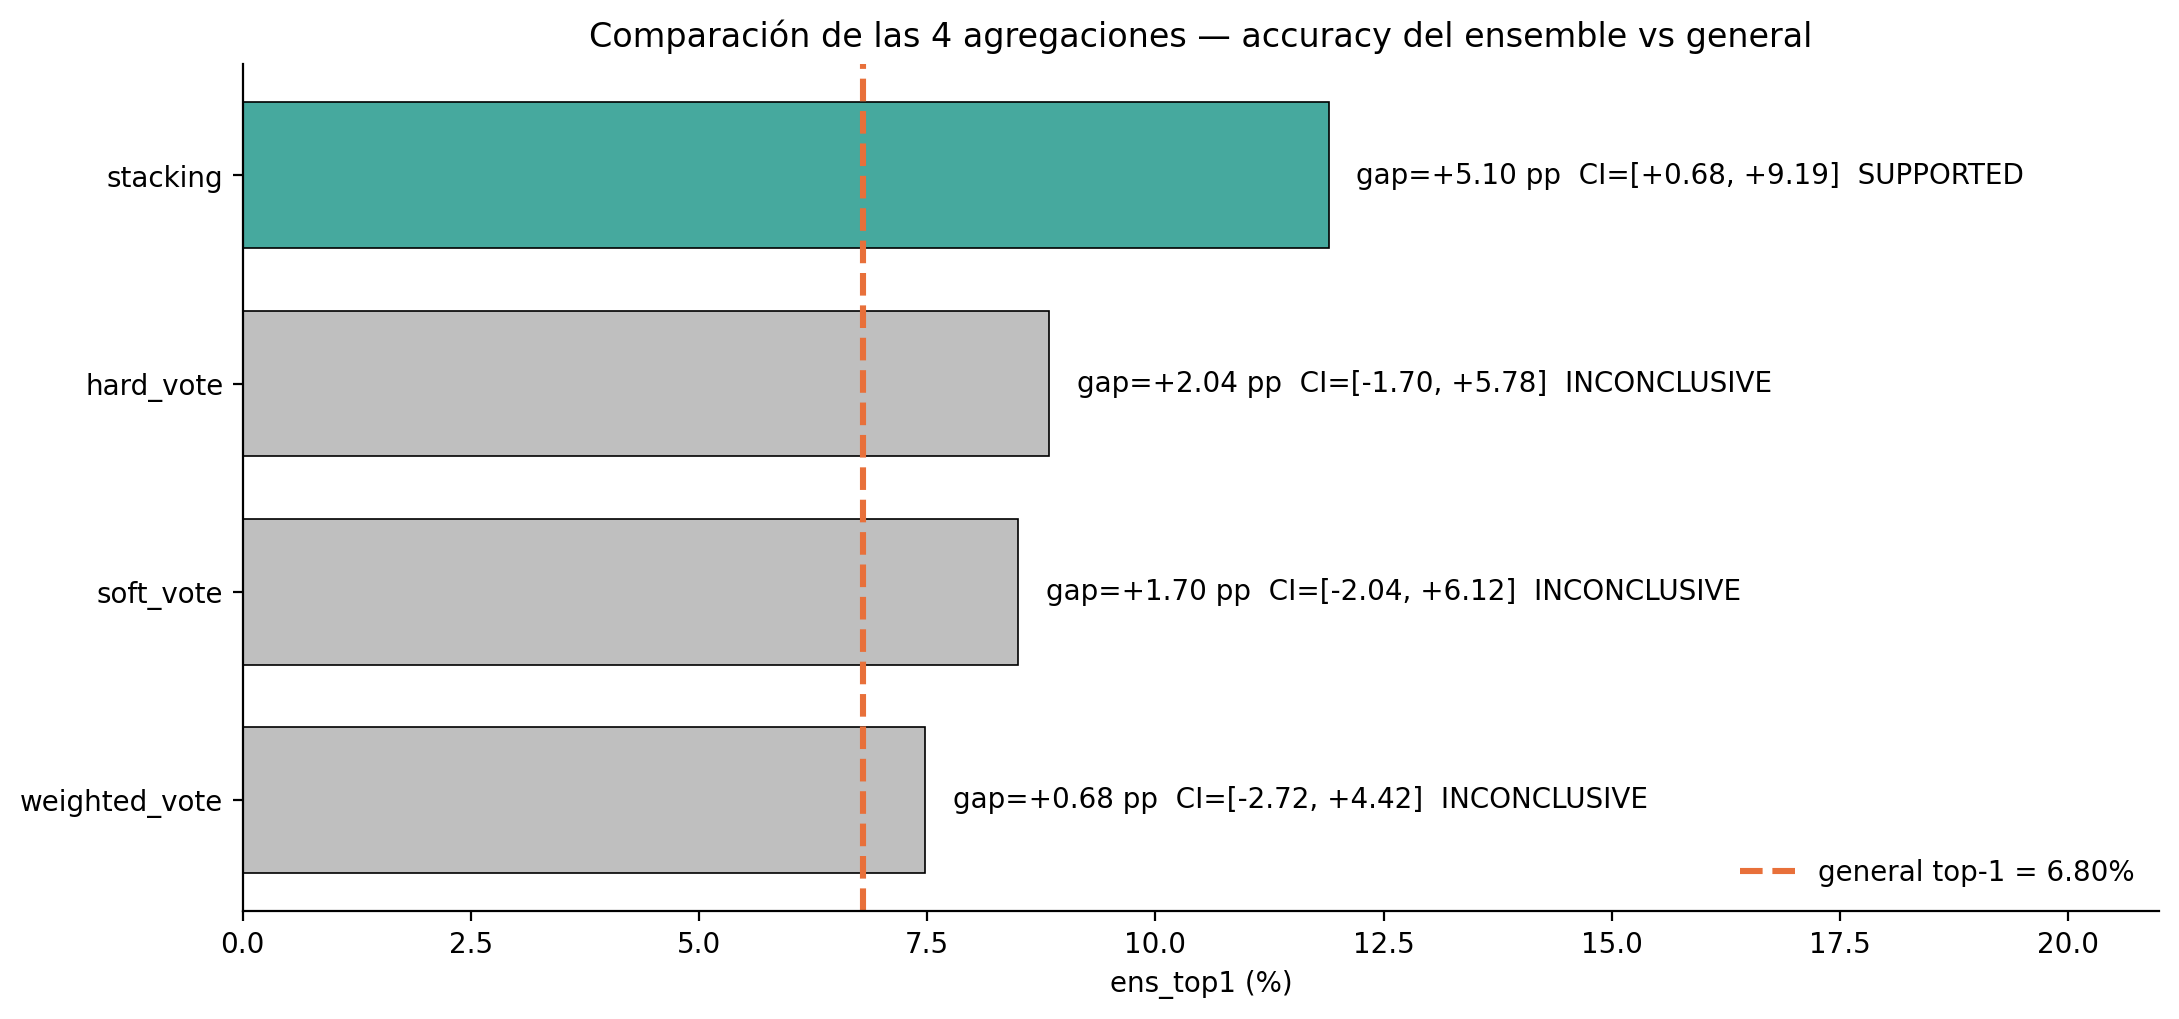
\includegraphics[width=0.72\linewidth]{fig2_aggregations.png}
  \caption{Exactitud del conjunto según la forma de combinar predicciones. La
  línea naranja marca la exactitud del modelo único (6.80\,\%). Solo el
  apilamiento (verde) lo supera con significancia formal.}
  \label{fig:aggregations}
\end{figure}

El apilamiento es la única estrategia cuyo intervalo no incluye el cero
($\text{CI}_\text{low}=+0.68$\,pp). Las tres votaciones quedan \emph{por debajo}
del modelo único en exactitud absoluta: promediar a ciegas las predicciones de
submodelos que vieron pocos datos termina perjudicando, salvo que un meta-modelo
aprenda a distinguir cuándo conviene escuchar a cada uno.

Como se evalúan cuatro formas de combinar, una corrección por comparaciones
múltiples (por ejemplo, Bonferroni con $\alpha=0.0125$) endurecería el umbral de
significancia, y el $\text{CI}_\text{low}=+0.68$\,pp del apilamiento es marginal
bajo ese criterio más estricto. Por eso la solidez del resultado no descansa en
un único test, sino en la convergencia de tres líneas de evidencia: (i) el
bootstrap del apilamiento es robusto ante 4 semillas independientes; (ii) las 9
mediciones del bucle son direccionalmente consistentes (todas positivas); y
(iii) los dos experimentos controlados (Sección~\ref{sec:ablations}) delimitan de
forma interpretable cuándo el efecto aparece y cuándo desaparece.

\paragraph{Robustez ante la semilla del bootstrap.} Para descartar que la
significancia del apilamiento sea un artefacto del muestreo aleatorio, repetimos
el cálculo del intervalo con 4 semillas independientes ($\{1337, 42, 7, 2024\}$):
el $\text{CI}_\text{low}$ se mantuvo positivo en los cuatro casos (entre $+0.68$ y
$+1.02$\,pp, veredicto SOPORTADO en todos), lo que confirma que el resultado es
una propiedad robusta de los datos.

% -----------------------------------------------------------------------
\section{¿Cuándo Funciona y Cuándo No?}
\label{sec:ablations}

La ventaja del conjunto no es universal. Dos experimentos controlados
(Tabla~\ref{tab:ablations}) muestran sus límites.

\subsection{Si la Red Base es Demasiado Pequeña}

Repetimos todo el flujo con una red base más chica ($d{=}128$). Aunque el modelo
único mejora en términos absolutos ($\text{exact}_\text{únic}{=}11.6\,\%$ frente a
$6.8\,\%$), el apilamiento ya no aporta nada: la brecha cae a cero y el intervalo
incluye el cero ($[-0.044,\,+0.044]$, RECHAZADO). Con menos capacidad, los
distintos tipos de cabeza no logran aprovechar señales independientes sobre las
mismas características: los submodelos convergen al mismo espacio funcional,
cometen errores parecidos, y el meta-modelo no encuentra ninguna combinación que
supere al mejor submodelo individual.

\subsection{Si Hay Pocas Clases}

Repetimos el flujo con 10 clases de K700 (1\,000 videos de clasificación, conjunto
reservado de 200, misma $d{=}192$). Con 10 clases el espacio es estrecho: el
reparto equilibrado le da a cada submodelo porciones muy parecidas, y todos
aprenden algo casi idéntico. Curiosamente, concentrar los datos en menos clases
hace al modelo único más fuerte ($\text{exact}_\text{únic}{=}22.5\,\%$, $2.25$
veces el azar de $1/10$), pero el conjunto no logra superarlo
($\Delta{=}-1.5$\,pp, IC $[-7.0,\,+5.0]$, RECHAZADO de forma concluyente: el
extremo superior $+5.0$ descarta cualquier efecto cercano al $+5.10$ observado con
30 clases).

\begin{table}[h]
\centering
\caption{Experimentos controlados (apilamiento): la ventaja del conjunto requiere
una red base con capacidad suficiente \emph{y} un espacio de clases amplio. En los
dos casos degradados el modelo único es más fuerte, pero el conjunto no lo supera.}
\label{tab:ablations}
\begin{tabular}{lcccc}
\toprule
\textbf{Variante} & $d$ & Clases & $\Delta$ & \textbf{Veredicto} \\
\midrule
\textbf{Principal} & \textbf{192} & \textbf{30} & $\mathbf{+5.10}$\,pp & \textbf{SOPORTADO} \\
Menor capacidad    & 128 & 30 & $+0.00$\,pp & RECHAZADO \\
Pocas clases       & 192 & 10 & $-1.50$\,pp & RECHAZADO \\
\bottomrule
\end{tabular}
\end{table}

% -----------------------------------------------------------------------
\section{Análisis}

\subsection{Por Qué el Apilamiento es Imprescindible}

Cuando todos los submodelos tienen la misma cabeza, sus predicciones se parecen
tanto que el meta-modelo no puede más que repetir el consenso, y la brecha se
desvanece (así ocurría en una versión homogénea previa, con brecha
$\approx 0$). La diversidad de cabezas cambia esto: la cabeza lineal capta señales
generales promediadas, la MLP agrega matices puntuales, y la atencional rescata la
estructura temporal. Como cada cabeza acierta y falla de manera distinta, el
apilamiento aprende pesos diferenciados sobre las $N{\times}C$ probabilidades y
aprovecha esa diversidad; las votaciones simples, que tratan a todos por igual, no
pueden hacerlo y quedan por debajo del modelo único.

\subsection{La Ventaja se Achica Cuando el Modelo Único Mejora}

La Fig.~\ref{fig:gap_vs_gen} relaciona la exactitud del modelo único con la brecha
a lo largo de las nueve mediciones.

\begin{figure}[t]
  \centering
  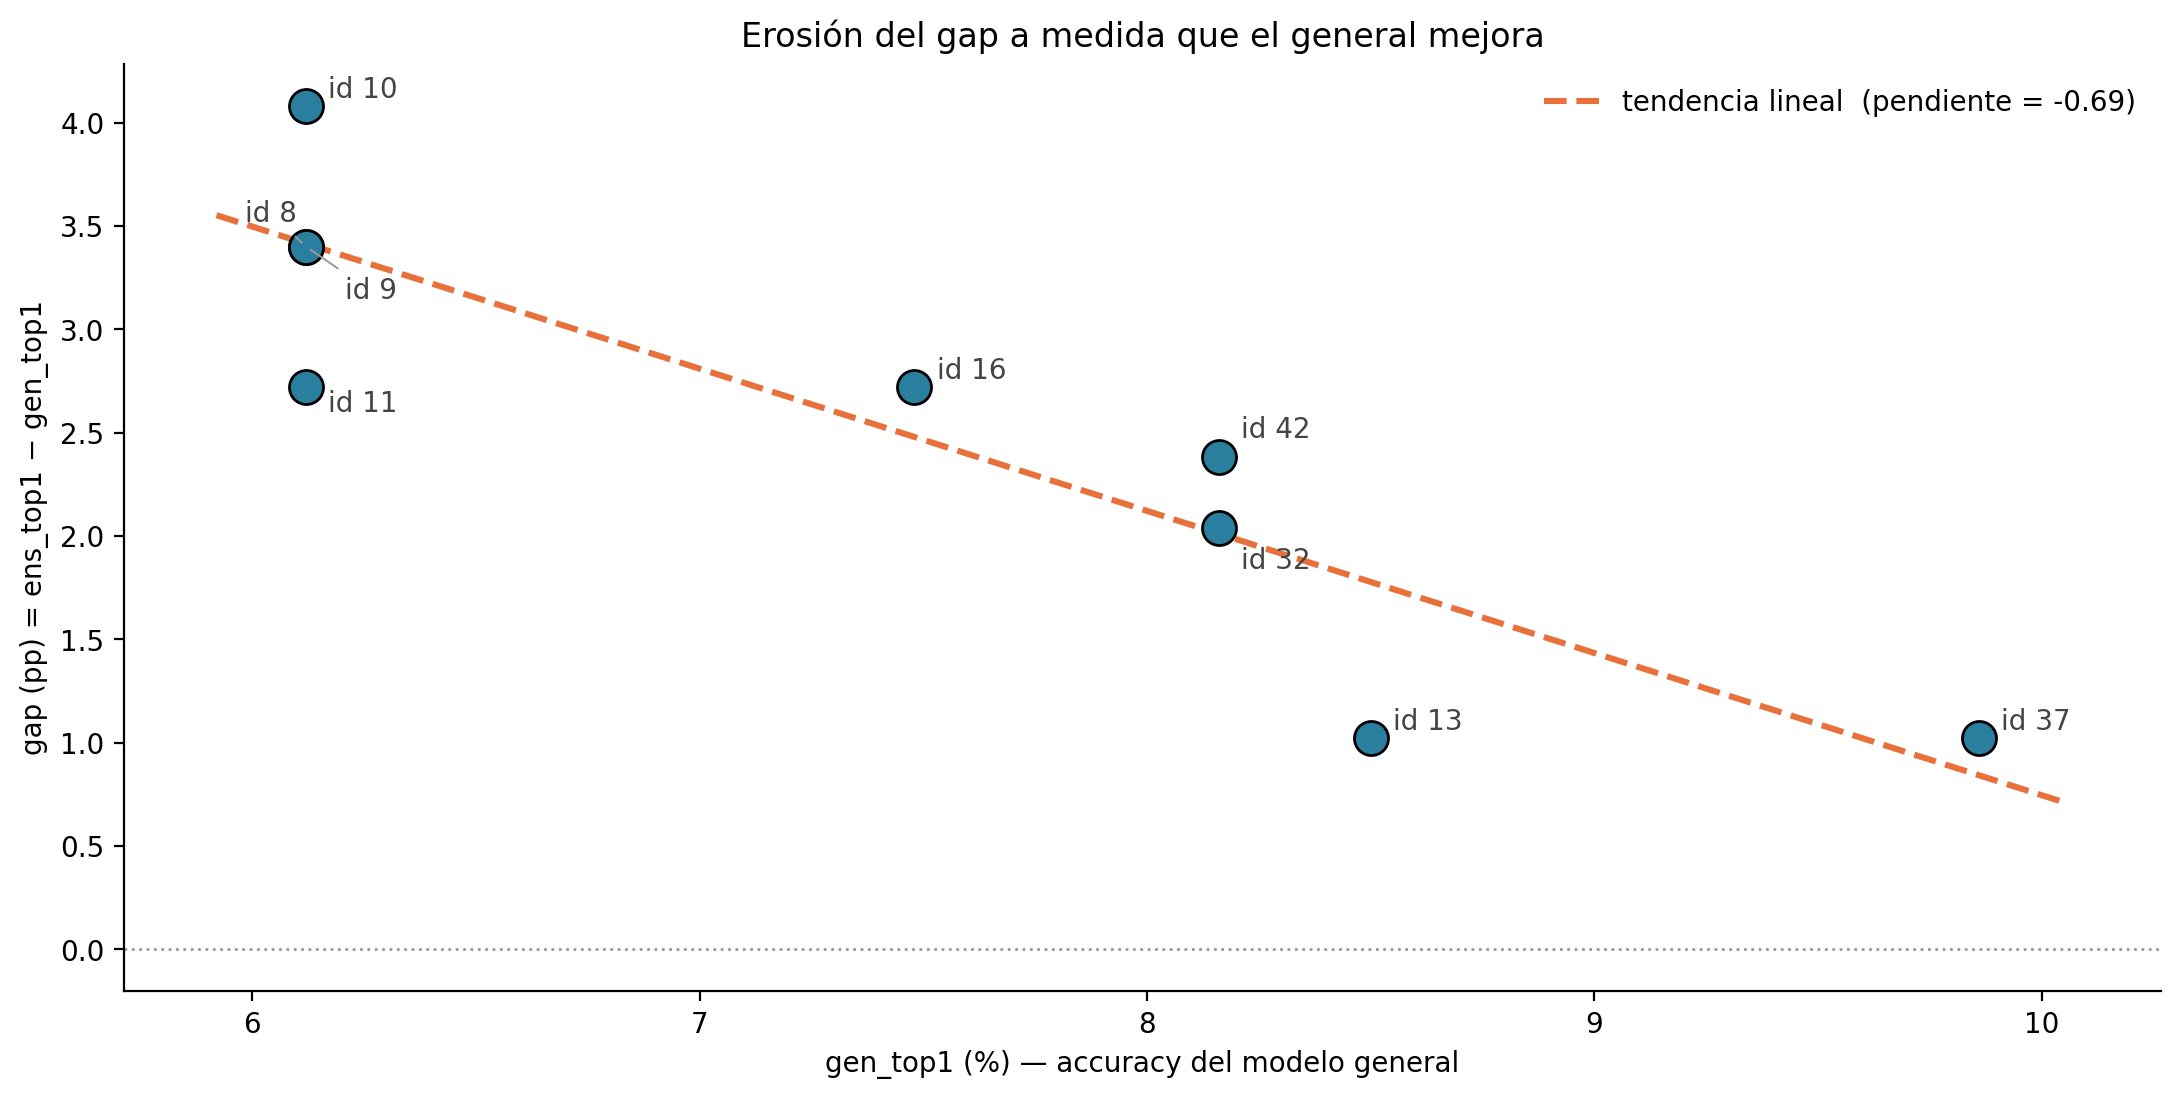
\includegraphics[width=0.72\linewidth]{fig3_gap_vs_general.png}
  \caption{La brecha se achica a medida que el modelo único mejora. Cada punto es
  una medición de la Fase 4. La tendencia es marcada (pendiente $\approx -0.69$,
  $R^2 \approx 0.80$): por cada punto que gana el modelo único, la brecha se
  reduce unos 0.69 puntos. Al ser una relación observacional sobre 9
  configuraciones, la pendiente debe leerse como tendencia, no como efecto causal.}
  \label{fig:gap_vs_gen}
\end{figure}

Tiene sentido: el modelo único ve todos los datos y aprovecha mejor cada mejora
del clasificador que un submodelo, que solo ve una porción. La ventaja del
conjunto es, entonces, más notoria cuando los modelos individuales son
relativamente débiles, en línea con lo observado en la
literatura~\cite{lakshminarayanan2017simple}.

\subsection{Las Dos Condiciones para que Funcione}

Los dos experimentos delimitan, juntos, las condiciones necesarias: una
\textbf{red base con capacidad suficiente} ($d \geq 192$; por debajo, los
submodelos no cometen errores distintos) y una \textbf{cantidad de clases
suficiente} ($C \geq 30$; con pocas clases, convergen a la misma solución).
Ninguna alcanza por sí sola: hacen falta ambas, junto con el apilamiento y la
evaluación sobre múltiples fragmentos.

% -----------------------------------------------------------------------
\section{Limitaciones}

\begin{enumerate}
  \item \textbf{Conjunto reservado chico} (294 videos, $\approx 0.34$\,pp por
        video): los intervalos de cada medición individual son anchos
        ($\approx 6$--$8$\,pp). La significancia es sólida en el promedio de las
        nueve mediciones y en la comparación directa entre formas de combinar.
        Un conjunto reservado de $\geq 1\,000$ videos daría más poder estadístico
        por medición.

  \item \textbf{Exactitudes absolutas bajas}: alrededor del 12\,\% sobre 30 clases
        ($\approx 3.6$ veces el azar de $1/30$), reflejo de la limitada calidad
        del codificador entrenado sobre solo 3\,000 videos. V-JEPA original usa
        unos 2 millones de videos ($\approx 670$ veces más), lo que ubica este
        trabajo en un régimen de cómputo y datos sumamente acotado.

  \item \textbf{Diversidad limitada a la cabeza}: todos los submodelos comparten
        el mismo codificador. Lograr codificadores realmente distintos exigiría
        varios entrenamientos sin etiquetas, fuera del alcance del hardware
        disponible.

  \item \textbf{Dependencia estadística y variabilidad de entrenamiento}: las nueve
        mediciones comparten el conjunto reservado y provienen del mismo bucle (no
        son independientes), y los resultados surgen de un único entrenamiento del
        codificador y de un único conjunto de submodelos. La única incertidumbre
        cuantificada es la del bootstrap; no se repitió el entrenamiento con varias
        semillas, por lo que la variabilidad de inicialización queda fuera de los
        intervalos.
\end{enumerate}

% -----------------------------------------------------------------------
\section{Conclusiones}

La hipótesis central de pico-JEPA ---un conjunto de modelos pequeños sobre
porciones de datos supera a un único modelo entrenado con todos los datos--- queda
\textbf{validada con significancia estadística formal} cuando concurren tres
condiciones: diversidad en la cabeza de clasificación, apilamiento como forma de
combinar, y evaluación sobre múltiples fragmentos. La brecha es de $+5.10$\,pp
(IC 95\,\% bootstrap $[+0.68,\,+9.19]$, robusto ante 4 semillas); además, las
nueve mediciones del bucle son direccionalmente consistentes
($\bar\Delta{=}+2.53$\,pp, todas positivas). Dos experimentos controlados marcan
los límites: la ventaja se anula con una red base de menor capacidad ($d{=}128$) o
con pocas clases (10), porque en ambos casos los submodelos convergen al mismo
espacio funcional y no generan la diversidad que el apilamiento explota.

Como trabajo futuro proponemos: (1) ampliar el conjunto de entrenamiento sin
etiquetas para mejorar la calidad del codificador ---medida por \emph{sondeo
lineal}, la exactitud de una única capa lineal entrenada sobre el codificador
congelado; objetivo: $> 25\,\%$---, lo que liberaría el techo de la clasificación;
(2) caracterizar cómo cambia la brecha entre 10 y 30 clases, para ubicar el punto
donde nace la ventaja; y (3) hacer lo mismo variando la dimensión $d$ de la red
base.

% -----------------------------------------------------------------------
% \section*{Agradecimientos}
%
% Agradecemos al proyecto K700 por los datos públicos.

% -----------------------------------------------------------------------
\bibliographystyle{splncs04}
{\footnotesize
\begin{multicols}{2}
\begin{thebibliography}{10}

\bibitem{lecun2022path}
Y.~LeCun,
``A path towards autonomous machine intelligence,''
\emph{OpenReview}, 2022.

\bibitem{assran2023self}
M.~Assran et al.,
``Self-supervised learning from images with a joint-embedding predictive
architecture,''
in \emph{CVPR}, 2023.

\bibitem{bardes2024revisiting}
A.~Bardes et al.,
``Revisiting feature prediction for learning visual representations from
video,''
\emph{arXiv:2404.08471}, 2024.

\bibitem{dietterich2000ensemble}
T.~G.~Dietterich,
``Ensemble methods in machine learning,''
in \emph{Multiple Classifier Systems}, Springer, 2000, pp.\ 1--15.

\bibitem{lakshminarayanan2017simple}
B.~Lakshminarayanan, A.~Pritzel, and C.~Blundell,
``Simple and scalable predictive uncertainty estimation using deep ensembles,''
in \emph{NeurIPS}, 2017.

\bibitem{wenzel2020hyperparameter}
F.~Wenzel et al.,
``Hyperparameter ensembles for robustness and uncertainty quantification,''
in \emph{NeurIPS}, 2020.

\bibitem{fort2019deep}
S.~Fort, H.~Hu, and B.~Lakshminarayanan,
``Deep ensembles: A loss landscape perspective,''
\emph{arXiv:1912.02757}, 2019.

\bibitem{wang2018temporal}
L.~Wang et al.,
``Temporal segment networks for action recognition in videos,''
\emph{IEEE Trans.\ Pattern Anal.\ Mach.\ Intell.}, vol.\ 41,
pp.\ 2740--2755, 2018.

\bibitem{jacobs1991adaptive}
R.~A.~Jacobs, M.~I.~Jordan, S.~J.~Nowlan, and G.~E.~Hinton,
``Adaptive mixtures of local experts,''
\emph{Neural Computation}, vol.\ 3, no.\ 1, pp.\ 79--87, 1991.

\bibitem{smaira2020short}
L.~Smaira et al.,
``A short note on the Kinetics-700-2020 human action dataset,''
\emph{arXiv:2010.10864}, 2020.

\bibitem{rostagno2025pico}
A.~Rostagno et al.,
``pico-JEPA: Comprendiendo el Video con Modelos Ultra-Ligeros y la
Sabiduría Colectiva,''
in \emph{XXXI Congreso Argentino de Ciencias de la Computación (CACIC)}, 2025.

\end{thebibliography}
\end{multicols}
}

\end{document}
